\documentclass[conference]{IEEEtran}
\usepackage[T1]{fontenc}
\usepackage{lmodern}
\usepackage{microtype}
\usepackage{amsmath,amssymb}
\usepackage{graphicx}
\usepackage{booktabs}
\usepackage{multirow}
\usepackage{tikz}
\usetikzlibrary{arrows.meta,positioning,fit,calc}
\usepackage{algorithm}
\usepackage{algorithmic}
\usepackage[hidelinks]{hyperref}
\usepackage{url}
\def\BibTeXdots{...}

% Fill in before submission.
\newcommand{\authorname}{Akif Jawad}
\newcommand{\authorid}{23i-0583}
\newcommand{\repourl}{\url{https://github.com/AKIF-jk/trialmatch}}
\newcommand{\adapterurl}{\url{https://huggingface.co/AkifJK/trialmatch-qwen2.5-1.5b-lora}}
\newcommand{\videourl}{\url{https://youtu.be/ii5_kt-9xic}}

\begin{document}

\title{TrialMatch: Criterion-Level Clinical Trial Eligibility Screening with a Fine-Tuned Qwen2.5-1.5B and Hand-Written KV-Cached, Tiled-Attention and Speculative Decoders}

\author{\IEEEauthorblockN{\authorname}
\IEEEauthorblockA{Generative AI, Assignment 2 (individual)\\
Student ID: \authorid\\
Code: \repourl\\
Demo Video: \videourl}}

\maketitle

\begin{abstract}
We build a system that reads a patient note and one trial eligibility criterion, then returns a label from the dataset's own category set and the IDs of the note sentences that support it. The model is Qwen2.5-1.5B-Instruct adapted with LoRA on the 37 training patients of the TrialGPT Criterion Annotations. On the 8 held-out test patients (206 criteria) the three fine-tuned seeds reach accuracy $0.696\pm0.011$ and macro-F1 $0.431\pm0.019$, against $0.626$ and $0.226$ for a per-type majority baseline, and $0.146$ and $0.121$ for the untuned model after a parsing repair. Evidence macro-F1 is $0.804\pm0.013$. The test split has no \emph{excluded} row, the rare classes are mostly missed, and the 95\% intervals over 8 patients are wide. We also implement, from model forward passes, a KV-cached greedy decoder, a tiled online-softmax attention backend, and a speculative decoder with a model draft and a prompt-lookup draft. Cached decoding matches uncached decoding token for token in float32 and is 1.0 to 15.7 times faster on a T4. The tiled attention matches the reference within $1.1\times10^{-6}$ in float32 and uses 16 times less temporary memory at 4096 tokens, but is slower than a fused kernel. Speculative decoding with a 0.5B draft is slower than greedy (0.59 to 0.98), because a draft step costs 0.8 of a target step on this GPU; prompt lookup is 1.4 to 1.76 times faster. Everything is served in a Gradio application with a live inference-comparison tab and report export. This is an educational prototype, not a clinical enrollment tool.
\end{abstract}

\begin{IEEEkeywords}
clinical trial matching, LoRA, KV cache, online softmax, speculative decoding, evidence retrieval
\end{IEEEkeywords}

\section{Introduction}
Deciding whether a patient meets a trial's eligibility criteria is slow manual work. Each trial lists many inclusion and exclusion criteria, and each criterion must be checked against a free-text note. A useful assistant must do more than output yes or no. It must keep the dataset's categories (including ``not enough information'' and ``not applicable''), point to the sentences it relied on, and never read a missing sentence as proof either way.

This report covers one individual project with six parts: (i) adapt an open-weight decoder to output a structured label and cited sentence IDs; (ii) evaluate labels and evidence on a fixed patient-grouped split that was untouched until the end; (iii) implement and verify a KV-cached decoding loop; (iv) implement and verify tiled online-softmax attention; (v) implement and measure greedy speculative decoding; (vi) wrap all of it in a browser application. We report the failures and the rejected options along with the results.

\textbf{Contributions.} (1) A fine-tuned 1.5B model whose test results, with caveats about the tiny test set, are reported once, after a recorded freeze. (2) Decoders written against the model's forward pass, with equivalence tests and measured cost models. (3) An honest negative result: model-based speculative decoding is slower than cached greedy here, and a measured cost model explains why. (4) A browser application with live decoding comparisons and report export.

\section{Related Work}
\textbf{Trial matching.} TrialGPT~\cite{trialgpt} matches patients to trials with GPT-4 in three steps (retrieval, criterion-level matching with explanations, and ranking), and released the criterion annotations we use. We study only the criterion-level step, with a small open model, and we never feed the dataset's GPT-4 predictions or explanations to the model.

\textbf{Architecture and model.} The Transformer~\cite{attention} is the base of all models here. Qwen2.5~\cite{qwen25} supplies a family of decoder models with grouped-query attention and a shared tokenizer, which makes a small draft for the large one possible. Phi-3-mini~\cite{phi3} is the alternative we tested and rejected.

\textbf{Adaptation.} LoRA~\cite{lora} trains low-rank updates on frozen weights. With 37 training patients, a few million trainable parameters are a better fit than full fine-tuning, and we compare it with unfreezing the last two layers.

\textbf{Efficient attention.} FlashAttention~\cite{flash} computes exact attention in tiles with a running softmax so the score matrix is never stored, and online normalizer calculation~\cite{online} is the underlying recurrence. We write the recurrence in PyTorch for correctness, not speed.

\textbf{Speculative decoding.} Leviathan et al.~\cite{leviathan} and Chen et al.~\cite{chen} show that a cheap draft can propose tokens that the target verifies in one pass without changing the output distribution. With greedy decoding, verification reduces to comparing arg-max tokens, which is what we implement. We also test prompt lookup (copying n-grams from the prompt as the draft), as available in the Transformers library~\cite{hf}.

\section{Materials and Methods}

\subsection{Dataset, split and leakage checks}
We use only \texttt{ncbi/TrialGPT-Criterion-Annotations} (revision \texttt{1cfcafde94}, licence field ``other''): 1,015 annotations, 53 patients, 103 trials, 356 inclusion and 659 exclusion criteria. We sort the patient IDs, shuffle them with \texttt{numpy.random.default\_rng(42)} and assign 37, 8 and 8 patients to train, validation and test. The split was fixed before any class count was inspected and is published as \texttt{splits/manifest.json} (patient IDs, annotation IDs, per-class counts, dataset revision, sha256 \texttt{357486d0}). Tests check that no patient is in two splits, that the manifest hash matches, and that test rows load only when \texttt{scripts/final\_eval.py} passes an explicit flag. Table~\ref{tab:split} gives the counts. The classes are very imbalanced: \emph{not excluded} dominates, and the test split has no \emph{excluded} row.

Annotation 883 has a null criterion text. It stays in the manifest, is flagged, and is dropped from training and metrics. The dataset's own \texttt{training} column conflicts with the required split (44 patients have mixed flags), so it is ignored. Columns \texttt{gpt4\_*} and \texttt{explanation\_correctness} are never used, and neither is \texttt{trial\_title}.

\begin{table}[t]
\centering\small
\caption{Split sizes and label counts (from \texttt{splits/manifest.json}). NEI is ``not enough information'', N/A is ``not applicable''. The training count includes the unusable annotation 883.}
\label{tab:split}
\resizebox{\columnwidth}{!}{% Counts from splits/manifest.json; train includes annotation 883 (null criterion), which training and metrics drop.
\begin{tabular}{lrrrrrrrr}
\toprule
Split & Patients & Rows & incl. & not incl. & excl. & not excl. & NEI & N/A \\
\midrule
train & 37 & 603 & 88 & 13 & 8 & 292 & 174 & 28 \\
val & 8 & 206 & 35 & 3 & 2 & 101 & 53 & 12 \\
test & 8 & 206 & 27 & 7 & 0 & 91 & 66 & 15 \\
\bottomrule
\end{tabular}
}
\end{table}

\subsection{Inputs, outputs and tokenization}
The prompt (Qwen ChatML, written by hand and checked equal to \texttt{apply\_chat\_template} for all 206 validation rows on both tokenizers) holds the numbered note (\texttt{0. \ldots\ 1. \ldots}), the criterion type, the criterion text and the label set for that type with a one-line definition of each label. Inclusion criteria allow \emph{included}, \emph{not included}, \emph{not enough information} and \emph{not applicable}; exclusion criteria replace the first two with \emph{excluded} and \emph{not excluded}. The target is one JSON object, evidence first:
\begin{center}\small\texttt{\{"evidence\_sentence\_ids":[0,2],"label":"included"\}}\end{center}
Only the assistant tokens contribute to the loss (prompt tokens are masked with $-100$). The longest example is 623 tokens and the limit is 2,048, so nothing is truncated. The encoder raises an error rather than truncate, so a truncation would fail loudly. Targets are at most 29 tokens.

\subsection{Model candidates and choice}
Table~\ref{tab:models} compares the candidates. Qwen2.5-1.5B-Instruct is the target: Apache-2.0, not gated, 28 layers, 12 query heads and 2 key/value heads, 32,768-token context, 1.54B parameters, about 3.1~GB in fp16. It fits a 16~GB T4 with room for LoRA training (7.4~GB peak at micro-batch 4). Phi-3-mini-4k (3.8B, MIT) was evaluated as the baseline alternative; it needed 8.8~GB just to generate on validation and was 4.4 times slower (160 s against 36 s). After the parsing repair it scored higher untuned than Qwen (macro-F1 0.229 against 0.125, Table~\ref{tab:baseval}), but it is 2.5 times larger, has no smaller model sharing its tokenizer to act as a draft, and does not leave room on a T4 for training at the batch sizes used here, so Qwen was kept. Qwen2.5-0.5B-Instruct is the draft: Apache-2.0, 24 layers, hidden size 896, 494M parameters, about 1~GB. Its \texttt{tokenizer.json} has the same sha256 as the target's and the vocabulary size is the same (151,936), so token IDs are interchangeable.

\begin{table}[t]
\centering\small
\caption{Model candidates. Memory is weights only in 16-bit.}
\label{tab:models}
\begin{tabular}{lrrll}
\toprule
Model & Params & Weights & Licence & Role \\
\midrule
Qwen2.5-1.5B-Inst. & 1.54B & 3.1 GB & Apache-2.0 & target \\
Qwen2.5-0.5B-Inst. & 0.49B & 1.0 GB & Apache-2.0 & draft \\
Phi-3-mini-4k-Inst. & 3.8B & 7.6 GB & MIT & rejected \\
\bottomrule
\end{tabular}
\end{table}

The grouped KV heads make the cache small: each key or value tensor per layer is $[B,2,T,128]$, so one token costs $2\times28\times2\times128\times2$ bytes $=28.7$~KB in fp16 for the target and 12.3~KB for the draft.

\subsection{Fine-tuning}
We train LoRA adapters on the attention projections \texttt{q,k,v,o} with $r=16$, $\alpha=32$, dropout 0.05, learning rate $2\times10^{-4}$ with a cosine schedule and 5\% warm-up, batch size 8 (micro-batch 4), 3 epochs, an fp16 frozen base with float32 adapter weights, a gradient scaler and gradient checkpointing. The loss is token-level cross-entropy on the answer tokens only. The checkpoint of each run is its best epoch by strict validation macro-F1. We compared on validation only: $r\in\{8,16,32\}$, evidence-first against label-first output, oversampling the two rarest labels four times, and LoRA against unfreezing the last two layers (one learning rate, $2\times10^{-5}$). The three leaders were rerun with seeds 42, 43, 44, and the config with the best mean validation macro-F1 (\emph{rare labels $\times4$}) was frozen in \texttt{configs/final.json}. A 0.5B draft adapter was trained with the same pipeline.

\subsection{System architecture}
Fig.~\ref{fig:arch} shows the pipeline. A note is segmented into numbered sentences; each criterion is wrapped in the prompt; the fine-tuned model generates the JSON through the hand-written cached decoder (batches of 8, left-padded); the output is parsed, checked (label belongs to the criterion type, IDs inside the note) and turned into a result row. The default explanation is a template that quotes only the cited sentences. The overall outcome is an explicit rule, not a ground-truth label: any \emph{not included} or \emph{excluded} gives ``Likely ineligible''; otherwise any \emph{not enough information} gives ``Needs review''; otherwise ``Preliminarily eligible''. \emph{Not applicable} criteria do not count, and an unreadable output counts as ``Needs review''.

\begin{figure}[t]
\centering
\resizebox{\columnwidth}{!}{%
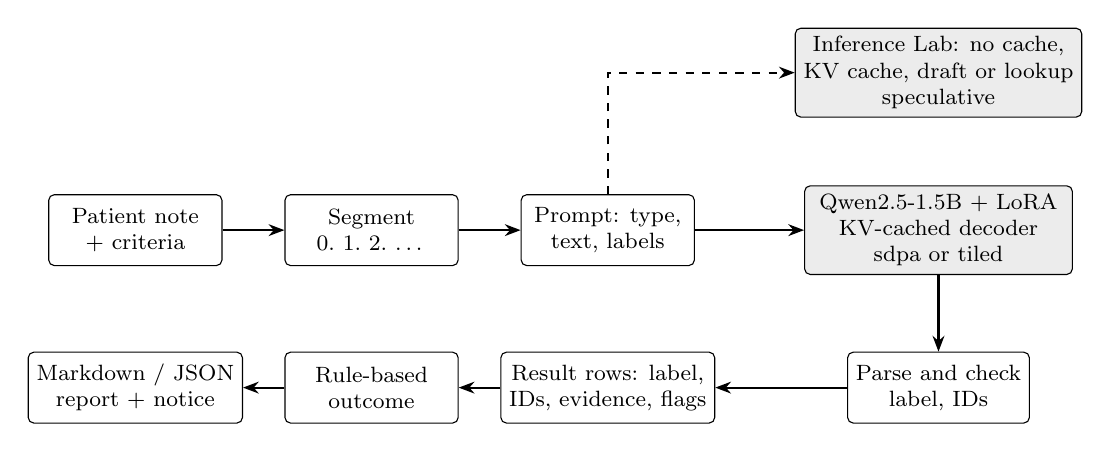
\begin{tikzpicture}[font=\footnotesize,
  box/.style={draw, rounded corners=2pt, align=center, minimum height=9mm, minimum width=22mm, inner sep=3pt},
  arr/.style={-{Stealth[length=2mm]}, thick}]
\node[box] (note) at (0,0) {Patient note\\+ criteria};
\node[box] (seg) at (3,0) {Segment\\0.\ 1.\ 2.\ \ldots};
\node[box] (prompt) at (6,0) {Prompt: type,\\text, labels};
\node[box, fill=gray!15, minimum width=34mm] (dec) at (10.2,0) {Qwen2.5-1.5B + LoRA\\KV-cached decoder\\sdpa or tiled};
\node[box] (parse) at (10.2,-2) {Parse and check\\label, IDs};
\node[box] (res) at (6,-2) {Result rows: label,\\IDs, evidence, flags};
\node[box] (agg) at (3,-2) {Rule-based\\outcome};
\node[box] (rep) at (0,-2) {Markdown / JSON\\report + notice};
\node[box, fill=gray!15, minimum width=34mm] (lab) at (10.2,2) {Inference Lab: no cache,\\KV cache, draft or lookup\\speculative};
\draw[arr] (note)--(seg); \draw[arr] (seg)--(prompt); \draw[arr] (prompt)--(dec);
\draw[arr] (dec)--(parse); \draw[arr] (parse)--(res); \draw[arr] (res)--(agg); \draw[arr] (agg)--(rep);
\draw[arr, dashed] (prompt.north) |- (lab.west);
\end{tikzpicture}}
\caption{System architecture. The screening path (solid) and the Inference Lab (dashed) run the same prompt through the same model.}
\label{fig:arch}
\end{figure}

\subsection{KV-cached decoding}
The reference path runs a full forward pass over all tokens at every step and keeps only the last column of logits. The cached path calls \texttt{model.forward} in an explicit loop with a \texttt{DynamicCache}: one prefill pass over the prompt, then one token per step. Both paths build their own 4-D mask (causal and padding) and their own positions. For left-padded batches the position of a token is $\mathrm{cumsum}(\text{mask})-1$, so padding does not shift rotary positions. After each step the loop asserts that the cache length equals the number of real tokens seen (the installed Transformers version takes no \texttt{cache\_position} for Qwen2, so this assertion replaces it). The cache grows by one token per layer per step, 28.7~KB per token for the target.

Numerical differences can arise because the two paths multiply tensors of different shapes, which changes the accumulation order. In fp16 this matters only when two top logits are within a couple of units in the last place.

\subsection{Tiled online-softmax attention}
The reference computes $\mathrm{softmax}(QK^\top/\sqrt{d})V$ with the full score matrix, a stable (max-subtracted) softmax and a bottom-right-aligned causal mask. The tiled version (Algorithm~\ref{alg:tiled}) loops over key tiles and keeps, per query row, a running maximum $m$, a normalizer $\ell$ and an unnormalized output $a$. When a tile raises the maximum, the old $\ell$ and $a$ are rescaled by $e^{m_\text{old}-m_\text{new}}$. Statistics are kept in float32 (float64 for float64 input). A row with no allowed key returns zeros in both functions, and a fully masked tile is handled by the same rule without a special case. Grouped KV heads are not copied: $Q$ is viewed as $[B,H_{kv},\text{rep},T_q,D]$ and the matrix product broadcasts over \texttt{rep}. The function is registered as a named attention backend of the model, so it can replace \texttt{sdpa} inside all 28 layers.

\begin{algorithm}[t]
\caption{Tiled attention with online softmax (one head)}
\label{alg:tiled}
\begin{algorithmic}[1]
\STATE $m\gets-\infty,\ \ell\gets0,\ a\gets0$ \COMMENT{per query row}
\FOR{each key tile $(K_j,V_j)$ of size $B_c$}
  \STATE $S\gets QK_j^\top/\sqrt{d}$; apply mask (set disallowed to $-\infty$)
  \STATE $m'\gets\max(m,\ \mathrm{rowmax}(S))$
  \STATE $P\gets\exp(S-m')$ (zero where $m'=-\infty$)
  \STATE $\alpha\gets\exp(m-m')$ (zero where $m'=-\infty$)
  \STATE $\ell\gets\alpha\ell+\mathrm{rowsum}(P)$;\ \ $a\gets\alpha a+PV_j$;\ \ $m\gets m'$
\ENDFOR
\STATE \textbf{return} $a/\ell$ (zeros where $\ell=0$)
\end{algorithmic}
\end{algorithm}

\subsection{Speculative decoding}
Algorithm~\ref{alg:spec} gives one round (batch size 1, greedy). The target cache holds all tokens but the last. The draft proposes up to $k$ tokens; the target reads the last token plus the proposals in one pass; the longest prefix of $m$ proposals that equal the target's arg-max tokens is accepted, and the target's next token is appended (a correction if $m<k$, a bonus token if $m=k$). Both caches are cropped to the accepted prefix, and the draft is fed the tokens it has not read. $k$ is capped by the tokens left, and a stop token ends the output at its first occurrence. A draft may propose fewer than $k$ tokens or none; a round without a proposal is a plain step. The two drafts are the 0.5B model (base or with its own LoRA adapter) and prompt lookup: the last 3, 2, or 1 tokens are searched for in the text so far (longest first, most recent match), and the tokens that followed are proposed.

\begin{algorithm}[t]
\caption{One greedy speculative round}
\label{alg:spec}
\begin{algorithmic}[1]
\STATE draft proposes $d_1\ldots d_k$ from the sequence $s$
\STATE target pass over $[s_{-1},d_1,\ldots,d_k]\Rightarrow$ arg-max tokens $t_0\ldots t_k$
\STATE $m\gets$ largest $m\le k$ with $d_i=t_{i-1}$ for all $i\le m$
\STATE append $d_1\ldots d_m$ and $t_m$ to $s$ (stop at a stop token)
\STATE crop the target cache to $s$ minus its last token; truncate the draft cache likewise
\end{algorithmic}
\end{algorithm}

\begin{figure}[t]
\centering
\resizebox{\columnwidth}{!}{%
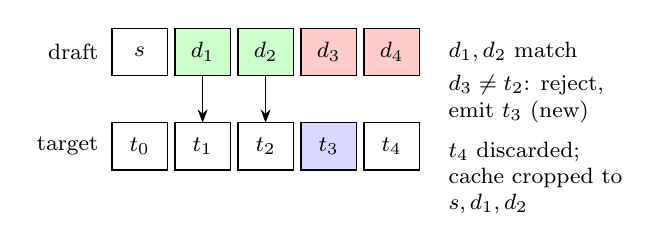
\begin{tikzpicture}[font=\footnotesize,
  tok/.style={draw, minimum width=7mm, minimum height=6mm, inner sep=1pt},
  ok/.style={tok, fill=green!20}, bad/.style={tok, fill=red!20}, new/.style={tok, fill=blue!15}]
\node[left] at (0,1.2) {draft};
\node[tok] (s) at (0.4,1.2) {$s$};
\node[ok] at (1.2,1.2) {$d_1$}; \node[ok] at (2.0,1.2) {$d_2$}; \node[bad] at (2.8,1.2) {$d_3$}; \node[bad] at (3.6,1.2) {$d_4$};
\node[left] at (0,0) {target};
\node[tok] at (0.4,0) {$t_0$}; \node[tok] at (1.2,0) {$t_1$}; \node[tok] at (2.0,0) {$t_2$}; \node[new] at (2.8,0) {$t_3$}; \node[tok] at (3.6,0) {$t_4$};
\draw[-{Stealth}] (1.2,0.9)--(1.2,0.3); \draw[-{Stealth}] (2.0,0.9)--(2.0,0.3);
\node[align=left, right] at (4.2,1.2) {$d_1,d_2$ match};
\node[align=left, right] at (4.2,0.6) {$d_3\neq t_2$: reject,\\emit $t_3$ (new)};
\node[align=left, right] at (4.2,-0.4) {$t_4$ discarded;\\cache cropped to\\$s,d_1,d_2$};
\end{tikzpicture}}
\caption{A speculative round with $k=4$ and $m=2$. Green proposals are accepted, red are rejected; $t_3$ is the correction token.}
\label{fig:specround}
\end{figure}

\subsection{Application}
The Gradio~\cite{gradio} application (\texttt{app.py}) has a \emph{Screening} tab and an \emph{Inference Lab} tab. Screening takes a pasted note (segmented into editable numbered sentences), criteria typed one per line or fetched from ClinicalTrials.gov by NCT ID (public trial metadata only), and returns for each criterion the label, cited IDs, highlighted evidence text, missing-information flags and an explanation, then the rule-based outcome. An optional model rationale is clearly labelled and receives only the cited sentences. Inputs are validated (empty note, broken numbering, more than 80 sentences or 8,000 characters, more than 12 criteria, empty or oversize criteria, unreadable model output) and each failure gives a plain message. Reports export as Markdown and JSON with the model and adapter revisions, decode settings, device, timestamp and the notice ``Educational screening prototype, not a clinical enrollment decision.'' The Inference Lab runs one prompt live through no cache, KV cache, model-draft speculative and lookup speculative decoding, with a chosen $K$ and attention backend (sdpa or tiled with tile 16, 64 or 256), compares every output with the cached reference, and shows prefill, decode, total time, tokens per second, peak extra memory, acceptance and target passes from that run. The text below the table is generated from the measured rows. Fig.~\ref{fig:shots} shows both tabs.

\begin{figure*}[t]
\centering
\IfFileExists{figures/app_screening.png}{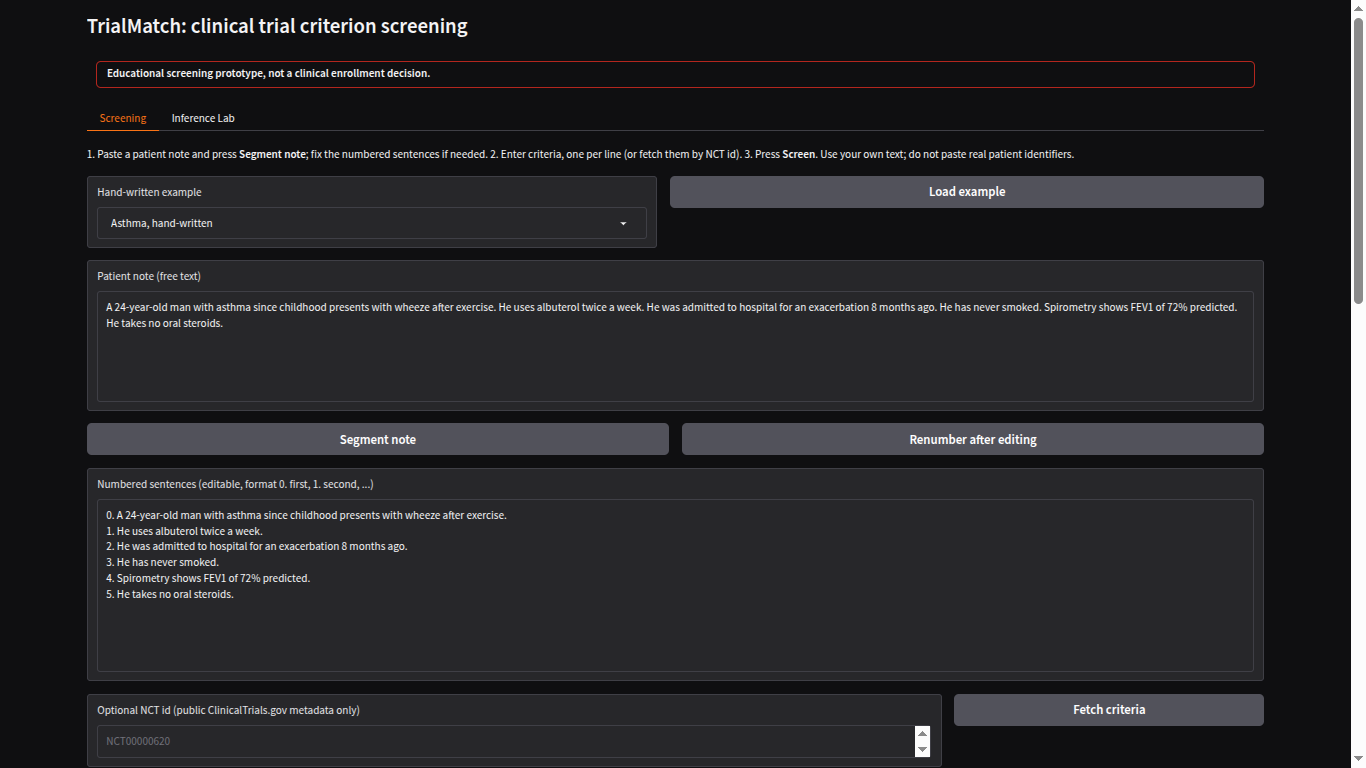
\includegraphics[width=0.48\textwidth]{figures/app_screening.png}}{\fbox{\parbox{0.45\textwidth}{\centering\vspace{3cm}[insert screenshot: Screening tab]\vspace{3cm}}}}\hfill
\IfFileExists{figures/app_lab.png}{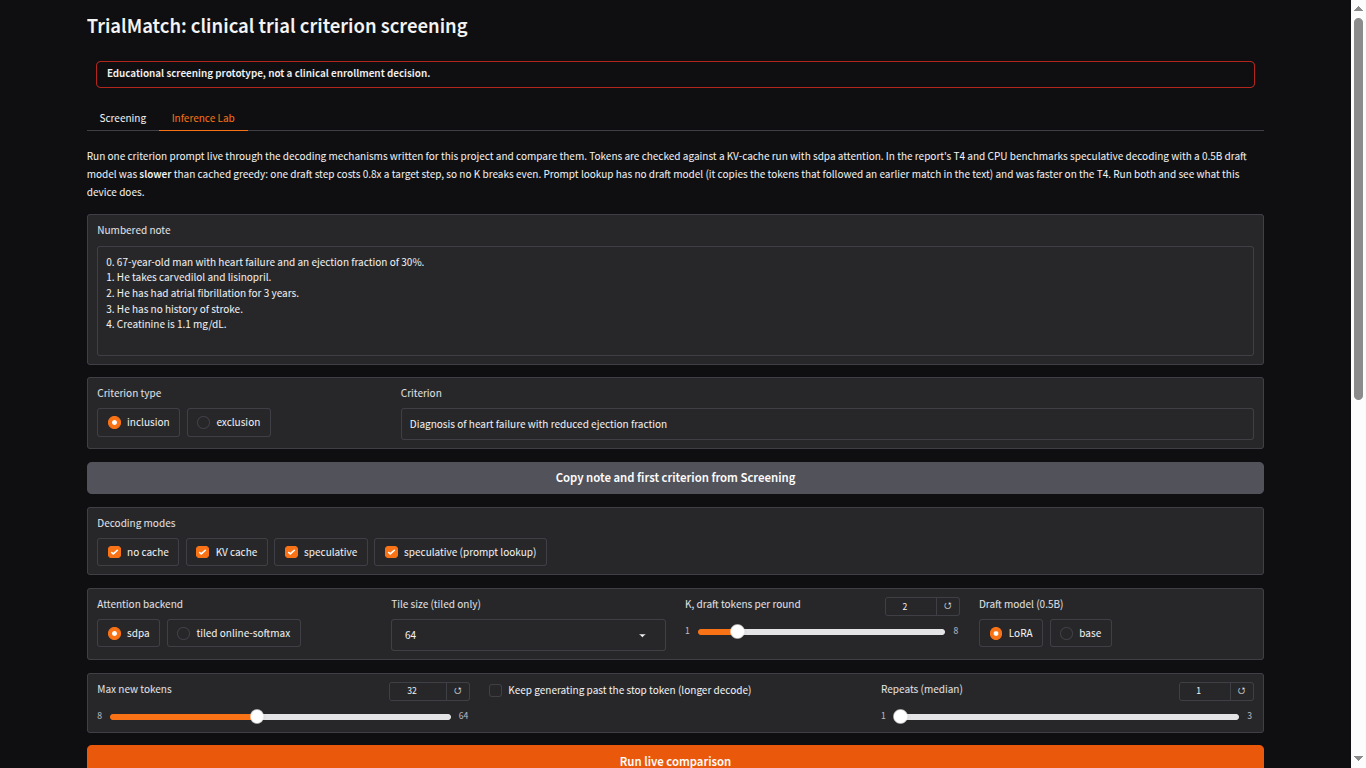
\includegraphics[width=0.48\textwidth]{figures/app_lab.png}}{\fbox{\parbox{0.45\textwidth}{\centering\vspace{3cm}[insert screenshot: Inference Lab tab]\vspace{3cm}}}}
\caption{Application screenshots: the Screening tab with per-criterion labels, cited sentences and the rule-based outcome (left), and the Inference Lab with a live four-mode comparison (right).}
\label{fig:shots}
\end{figure*}

\section{Experimental Setup and Metrics}
\textbf{Hardware.} Training and all GPU measurements ran on Kaggle Tesla T4 GPUs (16~GB, about 14.6~GB usable) through batch kernels; CPU measurements used 2 threads of a 4-CPU Kaggle host. The author's laptop (7~GB RAM, no GPU) was used only for code, documents and small result files. Each job records its commit, library versions and hardware; the software stack is PyTorch with Transformers 5.16.1 and PEFT.

\textbf{Decoding.} All comparisons use greedy decoding with \texttt{do\_sample=False} and \texttt{repetition\_penalty=1.0} set explicitly, because both Qwen models default to sampling with a penalty of 1.1. Evaluation uses fp16, batch 16 and at most 96 new tokens; the adapter is attached unmerged.

\textbf{Label metrics.} Accuracy, macro-F1 over the fixed six-label list, per-class precision, recall and F1, and confusion matrices, overall and split into inclusion and exclusion rows. A class with no support or no prediction scores 0 (zero-division rule fixed before the test run), and support is reported beside every class score. Because \emph{excluded} has no test row, the six-label macro-F1 cannot exceed 0.833, so we also report the average over the five supported labels.

\textbf{Evidence metrics.} Micro and macro precision, recall and F1 over sentence IDs. If gold and prediction are both empty, the record scores 1 in the macro average. If the prediction is empty and gold is not, recall is 0; if the prediction is non-empty and gold is empty, precision is 0. We also report macro-F1 on non-empty gold records. An ID outside the note is a false positive. Absent evidence never implies a label.

\textbf{Malformed output.} Strict parsing is the default and counts a malformed JSON object as a wrong prediction. One logged repair (take the first JSON object in the text) is reported separately and applies to the untuned baseline only; the fine-tuned model produced no malformed output.

\textbf{Test discipline.} The code, prompts and checkpoints were frozen and tagged (\texttt{final-freeze}, with sha256 of 17 files recorded). The test split was opened once, by a script that refuses to run unless the files match the record. We did not tune after seeing it. Confidence intervals resample the 8 test patients with replacement (1,000 draws).

\textbf{Timing.} Warm-up, \texttt{torch.cuda.synchronize()}, five repeats (three for speculative), median and inter-quartile range, with tokens checked equal.

\section{Results and Discussion}

\subsection{Validation: baselines, sweep and seeds}
Table~\ref{tab:baseval} shows the untuned models on the 206 validation rows. With strict parsing, Qwen2.5-1.5B scores 0.015 macro-F1, because it wraps 97 answers in a code fence; Phi-3-mini appends text to 64. After the repair step Qwen reaches 0.125 and Phi-3 0.229, and neither beats the per-type majority baseline on accuracy (0.621). Qwen predicts \emph{excluded} for 140 rows, so the untuned model is poor, not only badly formatted. This leaves a large gap for fine-tuning.

\begin{table}[t]
\centering\small
\caption{Validation, untuned models and the majority baseline (greedy, fp16, 206 rows).}
\label{tab:baseval}
\resizebox{\columnwidth}{!}{\begin{tabular}{llrrrr}
\toprule
Model & Parsing & Accuracy & Macro-F1 & Evidence F1 & Malformed \\
\midrule
Majority class (per criterion type) & n/a & 0.621 & 0.215 & 0.563 & 0 \\
Qwen2.5-1.5B-Instruct & strict & 0.015 & 0.015 & 0.358 & 97 \\
Qwen2.5-1.5B-Instruct & repaired & 0.180 & 0.125 & 0.451 & 0 \\
Phi-3-mini-4k-instruct & strict & 0.184 & 0.141 & 0.293 & 64 \\
Phi-3-mini-4k-instruct & repaired & 0.417 & 0.229 & 0.565 & 0 \\
\bottomrule
\end{tabular}
}
\end{table}

Table~\ref{tab:sweep} gives the single-seed sweep and Fig.~\ref{fig:curves} the validation curves. Every LoRA run beats the baselines (macro-F1 0.30 to 0.44 against 0.215), and unfreezing the last two layers is worst (0.298; only one learning rate was tried). The differences among the top runs come almost entirely from \emph{not applicable} (support 12), which some runs never predict, so the single-seed ranking is unreliable. Table~\ref{tab:seeds} confirms this: label-first led at seed 42 (0.440) but scored 0.366 and 0.363 at seeds 43 and 44. We froze \emph{rare labels $\times4$} (mean 0.446, SD 0.024) by the rule set in advance, but it is not distinguishable from $r=32$ (0.434, SD 0.010), which was the steadier run. In the report this is a close call, not a clear win.

\begin{table}[t]
\centering\small
\caption{Validation sweep, seed 42, best epoch by macro-F1.}
\label{tab:sweep}
\resizebox{\columnwidth}{!}{\begin{tabular}{lrrrrrr}
\toprule
Run & Epoch & Accuracy & Macro-F1 & Evidence F1 & Malformed & Peak GB \\
\midrule
r=16 (base) & 2 & 0.738 & 0.362 & 0.723 & 0 & 7.4 \\
r=8 & 2 & 0.748 & 0.371 & 0.745 & 0 & 7.4 \\
r=32 & 3 & 0.728 & 0.428 & 0.741 & 0 & 7.5 \\
label first & 3 & 0.752 & 0.440 & 0.742 & 0 & 7.4 \\
rare labels x4 & 3 & 0.738 & 0.426 & 0.739 & 0 & 7.4 \\
last 2 layers & 2 & 0.675 & 0.298 & 0.621 & 0 & 8.6 \\
\bottomrule
\end{tabular}
}
\end{table}

\begin{table}[t]
\centering\small
\caption{Validation, three seeds for the top configurations (mean $\pm$ SD).}
\label{tab:seeds}
\resizebox{\columnwidth}{!}{\begin{tabular}{lrrrr}
\toprule
Config & Macro-F1 per seed & Macro-F1 & Accuracy & Evidence F1 \\
\midrule
rare labels x4 (chosen) & 0.426 / 0.440 / 0.473 & 0.446 $\pm$ 0.024 & 0.731 $\pm$ 0.011 & 0.739 $\pm$ 0.003 \\
r=32 & 0.428 / 0.446 / 0.429 & 0.434 $\pm$ 0.010 & 0.739 $\pm$ 0.016 & 0.737 $\pm$ 0.003 \\
label first & 0.440 / 0.366 / 0.363 & 0.390 $\pm$ 0.044 & 0.741 $\pm$ 0.010 & 0.744 $\pm$ 0.010 \\
\bottomrule
\end{tabular}
}
\end{table}

\begin{figure}[t]
\centering
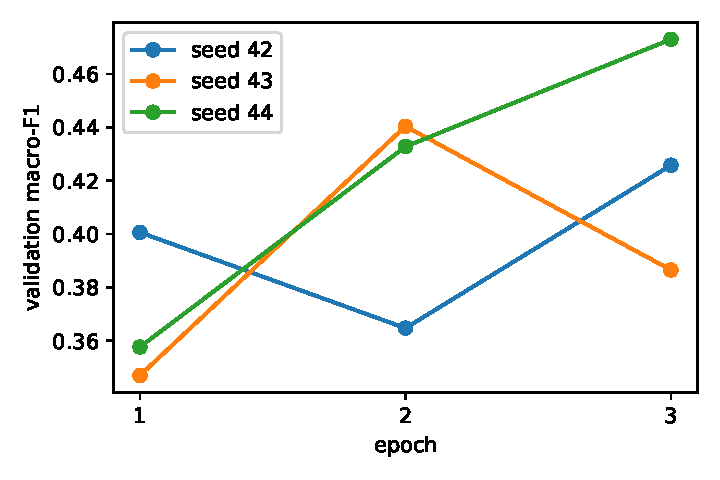
\includegraphics[width=\columnwidth]{figures/val_macro_f1_by_epoch.pdf}
\caption{Validation macro-F1 by epoch for the sweep runs. Most gains arrive in the first two epochs and the curves are noisy, which matches the small number of rare-class rows in validation.}
\label{fig:curves}
\end{figure}

\subsection{Held-out test}
Table~\ref{tab:test} is the single test run (206 rows, 8 patients; support: included 27, not included 7, excluded 0, not excluded 91, NEI 66, N/A 15). Fine-tuning moves the same model from 0.146 accuracy and 0.121 macro-F1 (repaired; 0.000 strict, 169 malformed outputs) to 0.696 and 0.431. The majority baseline has the best accuracy among the baselines (0.626), so the accuracy gain over it is 7 points. Table~\ref{tab:boot} shows that this gain is not established: the majority accuracy lies inside the intervals of all three seeds. The macro-F1 gain is clearer, since the lower interval ends (0.306 to 0.340) are above the upper end of the majority interval (0.277), though this compares two separately computed intervals and is not a paired test. Evidence macro-F1 is 0.804 against 0.704 for the empty-evidence baseline; evidence micro-F1 is 0.527, because the baseline predicts nothing and gets 0.000.

\begin{table*}[t]
\centering\small
\caption{Test results. The six-label macro-F1 is capped at 0.833 because \emph{excluded} has no test row; the five-label column averages the supported labels. ``Base'' is the untuned model with the same prompt and decoding.}
\label{tab:test}
% Test split, 206 rows, 8 patients; `excluded` has no test row, so Macro-F1 (5) averages the five supported labels.
\begin{tabular}{lrrrrrr}
\toprule
Model & Accuracy & Macro-F1 & Macro-F1 (5) & Evid. micro & Evid. macro & Malformed \\
\midrule
Majority class & 0.626 & 0.226 & 0.272 & 0.000 & 0.704 & 0 \\
Base, strict & 0.000 & 0.000 & 0.000 & 0.000 & 0.160 & 169 \\
Base, repaired & 0.146 & 0.121 & 0.145 & 0.153 & 0.320 & 3 \\
Fine-tuned, seed 42 & 0.709 & 0.436 & 0.523 & 0.522 & 0.791 & 0 \\
Fine-tuned, seed 43 & 0.689 & 0.410 & 0.492 & 0.539 & 0.817 & 0 \\
Fine-tuned, seed 44 & 0.689 & 0.447 & 0.536 & 0.521 & 0.804 & 0 \\
Fine-tuned, mean $\pm$ SD & 0.696 $\pm$ 0.011 & 0.431 $\pm$ 0.019 & 0.517 $\pm$ 0.023 & 0.527 $\pm$ 0.010 & 0.804 $\pm$ 0.013 & 0 \\
\bottomrule
\end{tabular}

\end{table*}

\begin{table}[t]
\centering\small
\caption{Test: 95\% intervals from resampling the 8 test patients.}
\label{tab:boot}
\resizebox{\columnwidth}{!}{% 95% percentile intervals from resampling the test patients with replacement (1000 draws).
\begin{tabular}{lrrr}
\toprule
Model & Accuracy & Macro-F1 & Evid. macro-F1 \\
\midrule
seed 42 & 0.709 [0.555, 0.827] & 0.436 [0.340, 0.509] & 0.791 [0.709, 0.857] \\
seed 43 & 0.689 [0.531, 0.807] & 0.410 [0.306, 0.486] & 0.817 [0.736, 0.887] \\
seed 44 & 0.689 [0.533, 0.799] & 0.447 [0.341, 0.527] & 0.804 [0.730, 0.874] \\
majority & 0.626 [0.461, 0.756] & 0.226 [0.164, 0.277] & 0.704 [0.628, 0.759] \\
\bottomrule
\end{tabular}
}
\end{table}

Validation to test, macro-F1 moves from 0.446 to 0.431 and accuracy from 0.731 to 0.696, a small drop and no sign of leakage. Table~\ref{tab:perclass} and Fig.~\ref{fig:conf} show where the model works: \emph{included} (F1 0.78, precision 1.00 for seed 44) and \emph{not excluded} (0.82) are good, \emph{not enough information} is moderate (0.58), and the rare classes are weak (\emph{not included} 0.22 with support 7, \emph{not applicable} 0.18 with support 15 and seed values 0.24, 0.00 and 0.32). No test row is \emph{excluded}, and the earlier validation hints that the oversampling might help the rare labels rest on one correct row each, so we make no claim about \emph{excluded}. Table~\ref{tab:bytype} scores inclusion and exclusion rows separately. Accuracy is similar (0.67 to 0.71 for inclusion, 0.70 to 0.71 for exclusion), but exclusion macro-F1 is lower (0.24 to 0.32 against 0.43 to 0.45) because the exclusion rows are dominated by \emph{not excluded} and contain no \emph{excluded} row. Evidence micro-F1 is also lower for exclusion (0.31 to 0.36 against 0.58 to 0.62), while evidence macro-F1 is higher (0.87 to 0.89 against 0.65 to 0.70), since many exclusion records have empty gold evidence and an empty prediction scores 1 there.

\begin{table}[t]
\centering\small
\caption{Test, per-class F1 for each seed, with seed-44 precision and recall.}
\label{tab:perclass}
\resizebox{\columnwidth}{!}{% Test split. `excluded` has support 0, so every value for it is 0 by the zero-division rule.
\begin{tabular}{lrrrrrrr}
\toprule
Label & Support & F1 s42 & F1 s43 & F1 s44 & F1 mean $\pm$ SD & P (s44) & R (s44) \\
\midrule
included & 27 & 0.800 & 0.773 & 0.773 & 0.782 $\pm$ 0.016 & 1.000 & 0.630 \\
not included & 7 & 0.167 & 0.286 & 0.211 & 0.221 $\pm$ 0.060 & 0.167 & 0.286 \\
excluded & 0 & 0.000 & 0.000 & 0.000 & 0.000 $\pm$ 0.000 & 0.000 & 0.000 \\
not excluded & 91 & 0.826 & 0.817 & 0.819 & 0.820 $\pm$ 0.005 & 0.710 & 0.967 \\
not enough information & 66 & 0.588 & 0.584 & 0.561 & 0.578 $\pm$ 0.014 & 0.667 & 0.485 \\
not applicable & 15 & 0.235 & 0.000 & 0.316 & 0.184 $\pm$ 0.164 & 0.750 & 0.200 \\
\bottomrule
\end{tabular}
}
\end{table}

\begin{table}[t]
\centering\small
\caption{Test, inclusion and exclusion rows scored separately (strict parsing). ``Supp.'' averages over labels with support.}
\label{tab:bytype}
\resizebox{\columnwidth}{!}{% Test split, strict parsing, inclusion and exclusion rows scored separately (macro-F1 over the six-label list; supp. = over labels with support).
\begin{tabular}{llrrrrrr}
\toprule
Model & Type & Rows & Accuracy & Macro-F1 & Macro-F1 (supp.) & Evid. micro F1 & Evid. macro F1 \\
\midrule
seed 42 & inclusion & 75 & 0.707 & 0.431 & 0.431 & 0.600 & 0.657 \\
seed 42 & exclusion & 131 & 0.710 & 0.295 & 0.393 & 0.316 & 0.868 \\
seed 43 & inclusion & 75 & 0.680 & 0.454 & 0.454 & 0.620 & 0.695 \\
seed 43 & exclusion & 131 & 0.695 & 0.236 & 0.315 & 0.314 & 0.887 \\
seed 44 & inclusion & 75 & 0.667 & 0.430 & 0.430 & 0.581 & 0.652 \\
seed 44 & exclusion & 131 & 0.702 & 0.315 & 0.420 & 0.357 & 0.891 \\
\bottomrule
\end{tabular}
}
\end{table}

\begin{figure}[t]
\centering
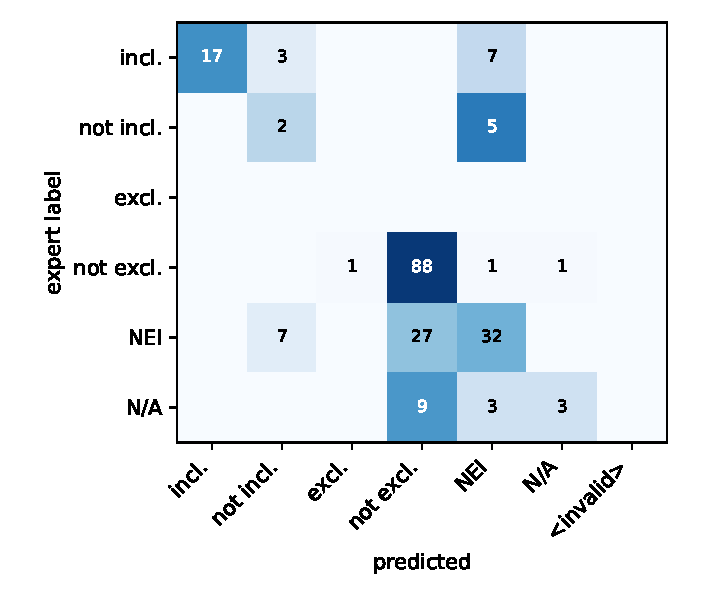
\includegraphics[width=0.8\columnwidth]{figures/confusion_test_seed44.pdf}
\caption{Test confusion matrix, seed 44 (the deployed adapter). The main off-diagonal mass is gold \emph{not enough information} predicted as \emph{not excluded}.}
\label{fig:conf}
\end{figure}

\subsection{Error analysis}
Label errors per seed are 60, 64 and 64 of 206, and 55 rows are wrong for all three seeds, so most errors are systematic. For seed 44 the largest group (27 of 64) is gold \emph{not enough information} answered \emph{not excluded}; with the 9 gold \emph{not applicable} rows answered \emph{not excluded}, 36 of 64 errors are exclusion criteria resolved as ``not excluded''. The model predicts \emph{not enough information} on only 2 exclusion rows, although the label makes up 17\% of the training exclusions. We did not test why; a closed-world habit (``nothing mentioned, so not excluded'') is a reading, not a finding. Ten distinct cases, with annotation IDs, are written up in \texttt{docs/error\_analysis.md}; the kinds are:

\begin{itemize}
\item \textbf{Missing information as absence} (ids 174, 193): for ``previous axillary surgery'' the experts mark \emph{not enough information} with no evidence and the model says \emph{not excluded}; for ``patients were moribund'' the experts cite five findings (tachycardia, blood pressure 80/60, \ldots) that do not settle it, and the model cites nothing.
\item \textbf{Rare classes} (ids 683, 693, 322, 162): two sleep-and-tonsillectomy exclusions are gold \emph{not applicable} and predicted \emph{not excluded}; a contraception exclusion for a 48-year-old man is gold \emph{not excluded} and seed 44 says \emph{not applicable}; for ``open aortic aneurysm repair'' the gold is \emph{not included} and the model says \emph{not enough information} while citing a groin mass. Five of the seven gold \emph{not included} rows end as \emph{not enough information}.
\item \textbf{Label contradicts its own evidence} (ids 186, 383, 176): the model cites the sentence the experts cite for ``heart rate of at least 90/min'' (``tachycardic'') and still answers \emph{not enough information}; for active lupus with a list of symptoms it cites joint pain and a facial rash and answers \emph{not included}; for ``no history of central vena catheterization'' it answers \emph{not included} with no citation.
\item \textbf{Unsupported or excess evidence} (ids 746, 184): a firm negative with nothing cited where the experts saw suggestive findings; and the only \emph{excluded} prediction of seed 44, for the catch-all ``other inappropriate situation''.
\end{itemize}

Evidence errors are smaller. Among the 142 rows where seed 44's label is right, it cites a sentence the experts did not on 13 rows, cites nothing where the experts cited something on 19 rows, and cites something where the experts cited nothing on 14. The experts themselves attach evidence to 17 of 66 \emph{not enough information} rows, so citing under that label is not always wrong. Seed 44 gives a decision label without any cited sentence on 3 rows. These cases support the rule that an empty evidence list never sets a label: it only raises a flag in the application.

\subsection{Unseen cases}
We wrote three patients and 26 criteria that are not in the dataset (a test checks the overlap) and ran the three seeds on them. The expected labels were written by the assistant and have not been reviewed by a clinician, so this is a sanity check, not a benchmark. Label accuracy is 14, 15 and 15 of 26 (0.54 to 0.58) and evidence macro-F1 is 0.83 to 0.87, with no malformed output. The failures repeat those on test: the three \emph{not enough information} exclusions are all answered \emph{not excluded}, and \emph{excluded} is never predicted even when the model cites the right sentence.

\subsection{KV-cached decoding}
The cached decoder matches the uncached reference in all 28 float32 records (3 prompt lengths $\times$ 3 output lengths $\times$ 2 prompts, left-padded batches and 32 validation rows with real stop tokens), with a maximum logit difference of $8.5\times10^{-4}$. In fp16, 25 of 28 records match. At the first differing step in the three failing cases all earlier tokens agree and the top two logits are within two fp16 units in the last place (0.0156 each in the range 16 to 32), so the cause is rounding at near ties and not a cache bug; the same inputs in float32 show no mismatch. Table~\ref{tab:decode} and Fig.~\ref{fig:decode} give the T4 timings. Cached decoding runs at 34 to 35 tokens/s for 64 and 256-token prompts and 32 to 34 for 1024-token prompts with long outputs (about 29 ms per token; short outputs at 1024 tokens give 25 to 32 because prefill counts), while uncached speed falls with sequence length, so the speedup grows from 1.0 (64 x 16) to 8.8 (1024 x 256) and 15.7 for a padded batch of 8. At a 64-token prompt the cache saves nothing, because the per-step cost is dominated by launch overhead (a guess consistent with the flat per-token time, not isolated). On the CPU, where cost grows with tokens processed, the speedup is 5.5 to 17.6 even for short prompts. The cache adds at most 0.06~GB peak memory in our cells. The size of the speedup varied between two T4 sessions (7.1 earlier against 8.8 here at 1024 x 256), because the uncached runs were 13 to 19\% slower on the second machine; the order of the results did not change.

\begin{table}[t]
\centering\small
\caption{T4 decoding benchmark, fp16, median of 5 runs. The ``no'' is the 64$\times$256 fp16 flip described in the text.}
\label{tab:decode}
\resizebox{\columnwidth}{!}{% Tesla T4, fp16, sdpa, median of 5 repeats (results/decoding/benchmark_cuda_float16).
\begin{tabular}{lrrrrrrl}
\toprule
Prompt x output & Batch & No cache s & KV cache s & Speedup & Cached tok/s & Peak GB & Tokens equal \\
\midrule
64 x 16 & 1 & 0.50 & 0.49 & 1.0 & 32.3 & 2.89 & yes \\
64 x 64 & 1 & 2.02 & 2.02 & 1.0 & 31.6 & 2.89 & yes \\
64 x 256 & 1 & 11.65 & 8.20 & 1.4 & 31.2 & 2.90 & no \\
256 x 16 & 1 & 1.01 & 0.50 & 2.0 & 32.1 & 2.91 & yes \\
256 x 64 & 1 & 4.28 & 2.00 & 2.1 & 31.9 & 2.91 & yes \\
256 x 256 & 1 & 19.39 & 8.04 & 2.4 & 31.9 & 2.91 & yes \\
1024 x 16 & 1 & 3.22 & 0.64 & 5.0 & 24.9 & 2.98 & yes \\
1024 x 64 & 1 & 13.14 & 2.14 & 6.2 & 30.0 & 2.98 & yes \\
1024 x 256 & 1 & 56.48 & 7.96 & 7.1 & 32.1 & 2.98 & yes \\
349 x 64 & 8 & 33.69 & 2.62 & 12.9 & 195.6 & 3.16 & yes \\
\bottomrule
\end{tabular}
}
\end{table}

\begin{figure}[t]
\centering
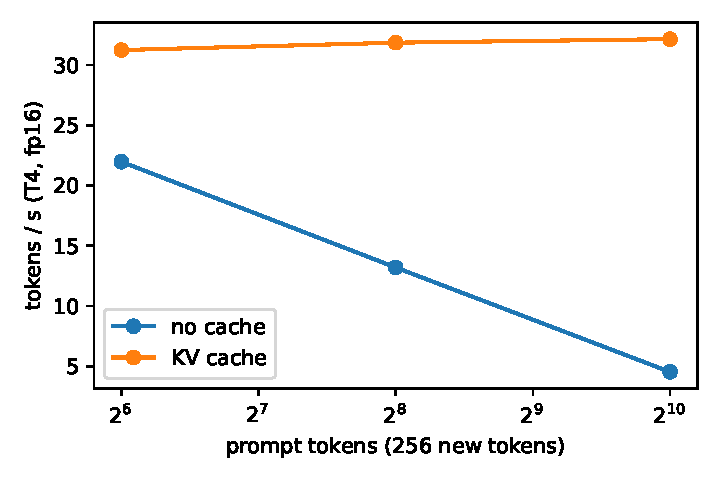
\includegraphics[width=\columnwidth]{figures/decode_tokens_per_second.pdf}
\caption{Decoding speed against prompt length: cached speed is flat, uncached speed falls.}
\label{fig:decode}
\end{figure}

\subsection{Tiled attention}
Against the float64 reference, 240 controlled cases (lengths 1, 7, 64, 256, 1024; tiles 1, 16, 64 and larger than $T$; six mask kinds; extreme scores) give a worst maximum error of $1.08\times10^{-6}$ in float32 (tolerance $10^{-5}$) and $2.1\times10^{-15}$ in float64 (tolerance $10^{-12}$), with no NaN (Table~\ref{tab:attnerr}). Negative controls (a naive softmax overflows, a wrong scale changes the output) fail as they should. End to end, the tiled backend inside the model gives identical tokens in 21 of 21 float32 cases and 19 of 21 in fp16; the two fp16 flips are an exact tie in the sdpa logits (28.53125) that the tiled path breaks by one or two units in the last place.

\begin{table}[t]
\centering\small
\caption{Tiled attention error against the float64 reference.}
\label{tab:attnerr}
\begin{tabular}{lrrr}
\toprule
Dtype & Cases & Worst max error & Tolerance \\
\midrule
float32 & 120 & 1.08e-06 & $10^{-5}$ \\
float64 & 120 & 2.11e-15 & $10^{-12}$ \\
\bottomrule
\end{tabular}

\end{table}

Table~\ref{tab:attnbench} and Fig.~\ref{fig:attn} give the cost. Tiling cuts temporary memory strongly: at $T=4096$ prefill the reference needs 2,345~MB and tile 64 needs 145~MB (16 times less). It is slower: 1.56 times the reference time at prefill and 22 times at a decode step with $T=4096$, because a decode step runs 64 loop iterations of several tiny kernels in each of 28 layers. The fused \texttt{sdpa} is fastest at prefill (53.4~ms against 70.8~ms) and does not save memory in this setup (1,896~MB). The reason is that a Python loop pays one kernel launch per operation per tile and moves each intermediate through GPU memory, while a fused kernel keeps tiles in on-chip memory in one launch, which a Python loop cannot do. Our function is a correctness and memory demonstration, not a speed path. End-to-end decode speed with the tiled backend was not benchmarked; in the application it ran slower than \texttt{sdpa} (1.05~s against 0.44~s for 13 tokens).

\begin{table}[t]
\centering\small
\caption{Attention benchmark on the T4 (fp16, 12 query heads, 2 KV heads, head dimension 128): median time and peak extra memory.}
\label{tab:attnbench}
\resizebox{\columnwidth}{!}{% Tesla T4, fp16, 12 query heads, 2 KV heads, head dim 128, median ms and peak extra MB.
\begin{tabular}{lrrrrrrr}
\toprule
Case & T & ms ref & ms tiled 64 & ms sdpa & MB ref & MB tiled 64 & MB sdpa \\
\midrule
prefill & 256 & 1.43 & 3.43 & 1.10 & 11 & 10 & 14 \\
decode & 256 & 1.17 & 2.39 & 0.78 & 3 & 0 & 5 \\
prefill & 1024 & 5.71 & 10.20 & 5.07 & 151 & 36 & 138 \\
decode & 1024 & 0.97 & 7.14 & 1.05 & 12 & 0 & 20 \\
prefill & 2048 & 17.65 & 29.28 & 13.84 & 592 & 73 & 500 \\
decode & 2048 & 1.05 & 13.32 & 1.17 & 24 & 0 & 40 \\
prefill & 4096 & 70.77 & 110.35 & 53.40 & 2345 & 145 & 1896 \\
decode & 4096 & 1.10 & 25.66 & 1.24 & 48 & 0 & 80 \\
\bottomrule
\end{tabular}
}
\end{table}

\begin{figure}[t]
\centering
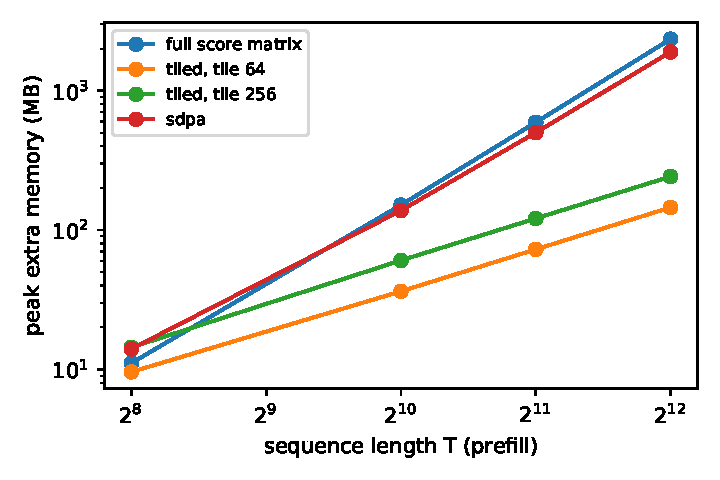
\includegraphics[width=\columnwidth]{figures/attention_peak_memory.pdf}
\caption{Peak extra memory against sequence length for the reference, tiled and \texttt{sdpa} attention.}
\label{fig:attn}
\end{figure}

\subsection{Speculative decoding}
Greedy equivalence holds in every test: stub drafts that always agree, always disagree and follow a script; a randomly initialised draft; the target as its own draft; stop tokens at several positions; a negative control without cache cropping, which fails as it should. On the real models, tokens equal cached greedy in 96 of 96 float32 cases and 160 of 160 fp16 cases (K $\in\{1,2,4,8\}$, base and LoRA draft), and HF assisted generation agrees in the 96 float32 cases. In the later benchmark, fp16 text generation flips 1 to 2 of 12 prompts in some cells (Table~\ref{tab:spec}); the benchmark keeps no logits, so we only note the same near-tie pattern as above and make no stronger claim.

Table~\ref{tab:spec} and Fig.~\ref{fig:spec} show the speed. With either 0.5B draft every setting is \emph{slower} than cached greedy: from 0.98 at best to 0.59 at worst. Acceptance is high for the fine-tuned draft on short JSON (0.97 at $K=1$, 0.63 at $K=8$) and the target passes fall (39 against 164 at $K=8$), yet each round costs more than the passes it replaces. We measured one draft step at 26 to 29~ms and one target pass at 33.5 to 35.6~ms, whatever $K$, so a round costs about $28K+35$~ms. For JSON, $K=2$ this gives $91.2$~ms and the measurement is $91.2$~ms; the round emits 2.81 tokens, i.e.\ 32.5~ms per token against 32.8~ms for greedy: break-even before prefill. The draft is 0.8 as costly as the target (24 layers against 28, launch bound), so no $K$ can win, and a larger $K$ lowers acceptance faster than it saves passes. The CPU gives the same sign (0.82 to 0.91 total; the reduced grid used one repeat), because a verification pass over 3 to 5 tokens costs about twice a one-token step.

Prompt lookup has no draft cost, and wins: 1.52 to 1.72 on JSON and 1.41 to 1.76 on free text for $K$ from 2 to 16, despite acceptance of only 0.09 to 0.56 and 24 to 46\% of rounds with no proposal. A round is one target pass (about 33~ms) plus 0.2~ms of lookup and emits about 1.9 tokens. On the CPU lookup is roughly break-even (0.83 to 1.10). The speedups come with a memory advantage too: the 0.5B draft adds about 1~GB of weights, lookup adds none, and peak extra memory above the loaded models was 25 to 34~MB in every cell.

\begin{table}[t]
\centering\small
\caption{Speculative decoding on the T4 (fp16, 12 validation rows, median of 3 repeats). Speedup is greedy cached total time over speculative total time.}
\label{tab:spec}
\resizebox{\columnwidth}{!}{% Tesla T4, fp16; speedup = greedy cached total time / speculative total time.
\begin{tabular}{llrrrrrr}
\toprule
Workload & Draft & K & Acceptance & Tokens/round & Target passes & Speedup & Prompts equal \\
\midrule
json & base & 1 & 0.939 & 1.85 & 94 & 0.90 & 12/12 \\
json & base & 2 & 0.907 & 2.81 & 66 & 0.94 & 12/12 \\
json & base & 4 & 0.661 & 3.38 & 57 & 0.75 & 12/12 \\
json & base & 8 & 0.558 & 5.07 & 42 & 0.64 & 12/12 \\
json & lora & 1 & 0.974 & 1.95 & 90 & 0.92 & 12/12 \\
json & lora & 2 & 0.935 & 2.81 & 66 & 0.93 & 12/12 \\
json & lora & 4 & 0.703 & 3.53 & 55 & 0.76 & 12/12 \\
json & lora & 8 & 0.634 & 5.63 & 39 & 0.71 & 12/12 \\
text & base & 1 & 0.810 & 1.80 & 645 & 0.93 & 11/12 \\
text & base & 2 & 0.723 & 2.43 & 481 & 0.87 & 11/12 \\
text & base & 4 & 0.618 & 3.44 & 358 & 0.77 & 11/12 \\
text & base & 8 & 0.427 & 4.34 & 270 & 0.59 & 12/12 \\
json & lookup & 2 & 0.555 & 1.67 & 103 & 1.52 & 12/12 \\
json & lookup & 4 & 0.429 & 1.92 & 91 & 1.71 & 12/12 \\
json & lookup & 8 & 0.216 & 1.92 & 91 & 1.71 & 12/12 \\
json & lookup & 16 & 0.108 & 1.92 & 91 & 1.67 & 12/12 \\
text & lookup & 2 & 0.401 & 1.61 & 785 & 1.40 & 10/12 \\
text & lookup & 4 & 0.283 & 1.81 & 668 & 1.63 & 11/12 \\
text & lookup & 8 & 0.173 & 1.95 & 623 & 1.74 & 11/12 \\
text & lookup & 16 & 0.090 & 1.90 & 612 & 1.74 & 11/12 \\
\bottomrule
\end{tabular}
}
\end{table}

\begin{figure}[t]
\centering
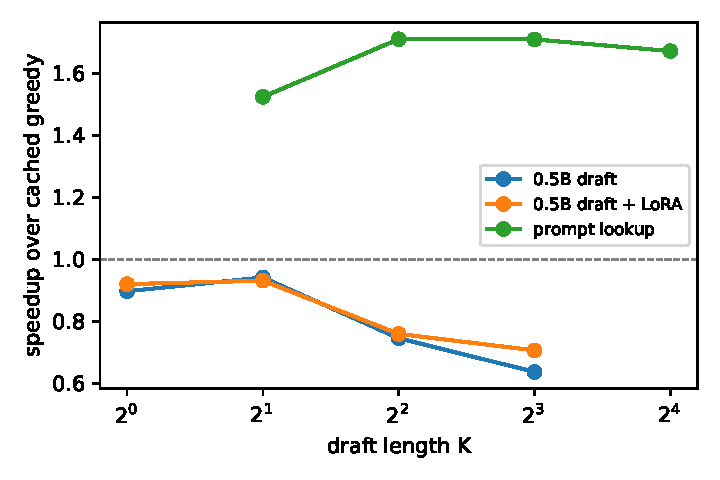
\includegraphics[width=\columnwidth]{figures/speculative_speedup.pdf}
\caption{Speedup over cached greedy by draft and $K$. Model drafts sit below 1, prompt lookup above.}
\label{fig:spec}
\end{figure}

\subsection{Application checks}
We ran the application on a Kaggle T4 behind a public tunnel and drove it from a browser. A hand-written diabetes example (7 criteria) screened in about 1 to 4~s, an asthma example (6 criteria, with rationale) in 3.1~s. An empty note gave ``Cannot run. The note is empty.'' and the next valid run worked; broken numbering and missing criteria gave plain messages and no stack trace. The Markdown and JSON reports carry the notice, the adapter folder and sha256, the greedy settings, device and timestamp. The Inference Lab returned the same tokens in all four modes with sdpa and with tiled attention, and reproduced the offline result: KV cache 1.2 to 1.8 times faster than no cache, model-draft speculative 0.86 to 1.04 times cached greedy, prompt lookup 1.2 to 1.7 (single short runs, so small gaps are noise). Labels on the hand-written examples were partly wrong (for example, an HbA1c of 8.1\% against a range of 7.5 to 11\% got \emph{not enough information}), in line with the modest scores above. Since the browser link dropped one event stream during the check, the page needs a reload ready during a demonstration.

\section{Limitations}
\begin{itemize}
\item \textbf{Small test set.} 8 patients and 206 rows; one patient moves several counts together, and the intervals are wide. The test split has no \emph{excluded} row, so that class is unmeasured, and the rare classes (\emph{not included}, \emph{not applicable}) are mostly missed.
\item \textbf{Weak abstention.} The model rarely says \emph{not enough information} for exclusion criteria, which is the unsafe direction for a screening tool.
\item \textbf{Model choice.} The frozen configuration beat the runner-up by half an SD of the seed noise; the choice was made by a rule set in advance, and may not be the best.
\item \textbf{Single annotator} per row in the data used, so ``wrong'' means ``differs from that annotation''. Some labels are debatable.
\item \textbf{Hosting.} Hugging Face refused to host a ZeroGPU Space for this account (HTTP 402 for ZeroGPU and for CPU hardware). The application therefore runs from a Kaggle notebook that prints a temporary public link, or with \texttt{python app.py} on any CUDA machine. There is no permanent URL, and the brief says an evaluator should not need to run a notebook; this is a known gap in the deliverable. The ZeroGPU code path was never run.
\item \textbf{Benchmarks.} T4 results come from two sessions on different machines; CPU benchmarks use a reduced grid, and the speculative CPU numbers use one repeat. The fp16 token flips were not isolated beyond near ties. HF assisted generation was checked in float32 only. Speculative decoding supports batch 1 and greedy decoding only.
\item \textbf{Clinical use.} The model was trained on 603 rows and the prompt allows no external knowledge. This is an educational prototype; the overall outcome is a rule on the labels, not a verdict.
\end{itemize}

\section{Conclusion}
A LoRA-adapted 1.5B model reaches test accuracy 0.696 and macro-F1 0.431 on criterion labels, with evidence macro-F1 0.804, clearly above the untuned model and the per-type majority baseline on macro-F1, but with wide intervals and unsolved rare classes and abstention. The hand-written cached decoder is token-identical to the uncached reference in float32 and up to 15.7 times faster on the T4; the tiled online-softmax attention is numerically correct and saves 16 times memory at 4096 tokens but loses to a fused kernel; and model-draft speculative decoding is correct but slower, for a reason we measured. Prompt lookup is the form of speculation that helps on this hardware. Future work: more patients or cross-validation, targeted data for exclusion abstention, a draft far cheaper than the target, and a permanent host.

\section*{Appendix: AI Use}
Claude Code (Anthropic) assisted with planning, implementation, Kaggle job management and drafting. The author reviewed and understands the code. Specifics are in \texttt{AI\_USE.md}; in particular, the expected labels of the hand-written unseen cases and the first draft of the error analysis and of this paper were written with the assistant's help, and all reused library code (Transformers, PEFT, Gradio) was exercised by tests. All numbers come from files under \texttt{results/}; tables and figures are regenerated by \texttt{scripts/make\_report\_assets.py}. Adapter weights: \adapterurl. Demo video: \videourl.

\begin{thebibliography}{10}
\bibitem{trialgpt} Q.~Jin \emph{et al.}, ``Matching patients to clinical trials with large language models,'' arXiv:2307.15051, 2023.
\bibitem{attention} A.~Vaswani \emph{et al.}, ``Attention is all you need,'' in \emph{Proc. NeurIPS}, 2017, arXiv:1706.03762.
\bibitem{qwen25} Qwen Team, ``Qwen2.5 technical report,'' arXiv:2412.15115, 2024.
\bibitem{phi3} M.~Abdin \emph{et al.}, ``Phi-3 technical report: A highly capable language model locally on your phone,'' arXiv:2404.14219, 2024.
\bibitem{lora} E.~J. Hu \emph{et al.}, ``LoRA: Low-rank adaptation of large language models,'' in \emph{Proc. ICLR}, 2022, arXiv:2106.09685.
\bibitem{flash} T.~Dao, D.~Y. Fu, S.~Ermon, A.~Rudra, and C.~R\'e, ``FlashAttention: Fast and memory-efficient exact attention with IO-awareness,'' in \emph{Proc. NeurIPS}, 2022, arXiv:2205.14135.
\bibitem{online} M.~Milakov and N.~Gimelshein, ``Online normalizer calculation for softmax,'' arXiv:1805.02867, 2018.
\bibitem{leviathan} Y.~Leviathan, M.~Kalman, and Y.~Matias, ``Fast inference from transformers via speculative decoding,'' in \emph{Proc. ICML}, 2023, arXiv:2211.17192.
\bibitem{chen} C.~Chen, S.~Borgeaud, G.~Irving, J.-B. Lespiau, L.~Sifre, and J.~Jumper, ``Accelerating large language model decoding with speculative sampling,'' arXiv:2302.01318, 2023.
\bibitem{hf} T.~Wolf \emph{et al.}, ``HuggingFace's Transformers: State-of-the-art natural language processing,'' arXiv:1910.03771, 2019.
\bibitem{gradio} A.~Abid, A.~Abdalla, A.~Abid, D.~Khan, A.~Alfozan, and J.~Zou, ``Gradio: Hassle-free sharing and testing of ML models in the wild,'' arXiv:1906.02569, 2019.
\end{thebibliography}

\end{document}
